\documentclass[11pt]{amsdtx}

\usepackage[scale=.7]{geometry}
\usepackage{bm}
\usepackage{amsrefs}     % 
\usepackage{amssymb}
\usepackage{amsmath}    % need for subequations
\usepackage[makeroom]{cancel} % for slashes through math terms
\usepackage{empheq}     % for boxing equations
\usepackage{graphicx}   % need for figures
\usepackage{verbatim}   % useful for program listings
\usepackage{color}      % use if color is used in text
\usepackage{listings}
%\usepackage{subfigure}  % use for side-by-side figures
%\usepackage{hyperref}   % use for hypertext links, including those to external documents and URLs
\raggedbottom           % don't add extra vertical space

\newcommand{\ud}{\mathrm{d}}
\newcommand{\bra}[1]{\left\langle #1 \right|}
\newcommand{\ket}[1]{\left| #1 \right\rangle}
\newcommand{\braket}[2]{\left\langle #1 | #2\right\rangle}
\newcommand{\mbf}[1]{\mathbf{\boldsymbol{#1}}}
\newcommand{\ddt}[1]{\frac{\ud #1}{\ud t}}
\newcommand{\st}{\mathrm{st}}
\newcommand{\nd}{\mathrm{nd}}
\newcommand{\rd}{\mathrm{rd}}
\newcommand{\nth}{\mathrm{th}}



\title{Direct collocation method for differential-algebraic equations (DAEs)}
\author{Vincent Chan}
\date{}


\begin{document}
\maketitle

The goal here is to solve differential-algebraic equations (DAEs) via the collocation method and somehow validate the solution.  With initial conditions and paramaters given, the specific DAE considered here is
\begin{eqnarray*}
%	\dot{x} &=& u \\
%	m\dot{u} &=& - f\dfrac{x}{l} \\
%	\dot{y} &=& v  \\
%	m \dot{v} &=& mg - f\dfrac{y}{l} \\
	m \dfrac{\ud^2 x}{\ud t^2} &=& -f\dfrac{x}{l} \\
	m \dfrac{\ud^2 y}{\ud t^2} &=& mg - f\dfrac{y}{l} \\
	0 &=& x^2 + y^2 - l^2 ~,
\end{eqnarray*}
and is equivalent to the ODE
\begin{eqnarray*}
	m \dfrac{\ud^2 \theta }{\ud t^2} + \dfrac{m g}{l} \sin \theta = 0~.
\end{eqnarray*}


The DAE can also be decomposed into a DAE of four $1^{\st}$-order ODEs plus an algebraic constraint:
\begin{eqnarray*}
	\dot{x} &=& u \\
	m\dot{u} &=& - f\dfrac{x}{l} \\
	\dot{y} &=& v  \\
	m \dot{v} &=& mg - f\dfrac{y}{l} \\
	0 &=& x^2 + y^2 - l^2 ~,
\end{eqnarray*}
again with the initial conditions and parameters given.

\section{Intro: deriving the derivative matrix}

Consider the expansion of an arbitrary (but smooth) function onto some orthogonal basis:
\begin{eqnarray}
	f(x) = \sum_{n = 0}^{\infty} a_n T_n(x)~,
\end{eqnarray}
for $x \in \left[ a, b \right]$.  Here, I actually have in mind for $\left\lbrace T_n(x) \right\rbrace$ the Chebyshev polynomials and $[a, b] = [-1, 1]$, but any set of orthogonal polynomials will serve as a basis.

In any of these orthogonal set of polynomials, $T_n(x)$ is a $n^{\nth}$-order polynomial.  As such, for well behaved functions, it is sufficient to consider only the first $N$ terms, for some natural number $N$:
\begin{eqnarray}
	f(x) = \sum_{n = 0}^{N} a_n T_n(x)~,
\end{eqnarray}
where the equality is kept because we've assumed any difference to be negligible.

Instead of $\left\lbrace T_n(x) \right\rbrace$ as the basis set, it is also possible to view $\left\lbrace a_n \right\rbrace$ as the basis set.  If we further consider $f$ at some $N+1$ points, then we can view the expansion as a linear transformation of one set of basis $\left\lbrace a_n \right\rbrace$ to another $\left\lbrace f_n \right\rbrace$:
\begin{eqnarray}
	f(x_n) = \sum_{m=0}^N T_m(x_n) a_m~,
\end{eqnarray}
or
\begin{eqnarray}
	\ket{f} = T(x) \ket{a}~.
\end{eqnarray}
%if you'd like to view the number of terms $N$ as being so large that we've recovered some compact subspace of $\mathbb{R}$.

Now, take the derivative of both sides with respect to $x$:
\begin{eqnarray}
	\dfrac{\ud}{\ud x} \ket{f} &=& \dfrac{\ud}{\ud x} \left( T(x) \ket{a} \right) \\
	\ &=& T'(x) \ket{a} \\
	\ &=& T'(x) T^{-1}(x) \ket{f}  \\
	\ &=& D \ket{f}~,
\end{eqnarray}
where we have now defined our derivative matrix $D(x) := T'(x) T^{-1}(x)$, a $(N+1) \times (N+1)$ matrix.

The only issue left is choosing the optimal set of points $\left\lbrace x_n \right\rbrace$ (note: these points are called \textbf{collocation points}.).  Without going into details (because I don't know the details), there are two supposed best choices for the collocation points:
\begin{enumerate}
	\item Gauss points, which are the zeros of the highest order polynomial, $T_N(x)$, and
	\item Gauss-Legendre points, where are the zeros of the derivative of the highest order polynomial, $T'_N(x)$ plus the boundary points (which varies depending on the choice of othogonal polynomials).
\end{enumerate}

For the purpose solving differential equations on a compact space (so that the problem of dealing with infinitly far away boundaries can be ignored), the Gauss-Legendre set of collocation points is the obvious choice.

\section{Ordinary Differential Equations}

To see how to utilize the derivative matrix $D$, it is simplest to give an example.  So consider
\begin{eqnarray}
	\dfrac{\ud y}{\ud x} = f(x)	~,
\end{eqnarray}
with initial condition $y(x_0) = y_0$.

Then we simply consider the truncated expansion and rewrite the problem as
\begin{eqnarray}
	D \ket{y} = \ket{f}~,
\end{eqnarray}
with IC $\ket{y}_{(x_0)} = y_0$.  At this point, should you try to solve for $\ket{y}$ as $\ket{y} = D^{-1}\ket{f}$, you'll come across the problem that $D$ is singular.  Of course, that is expected since there exists an infinite number of functions $y$ whose derivative is $f$.  So, we must find some way of incorporating the initial condition into the linear system of equations.  

The solution is to simply substitute the ODE for $\ket{y}(x_0)$ with the initial condition.  This gives us
\begin{eqnarray}
	\begin{pmatrix}
		1    & 0 & \cdots & 0 \\
		d_{10} & d_{11} & \cdots & d_{1N} \\
		\vdots & \vdots & \ddots & \vdots \\
		d_{N0} & d_{N1} & \cdots & d_{NN}
	\end{pmatrix}
	\begin{pmatrix}
		y(x_0) \\ y(x_1) \\ \vdots \\ y(x_N)
	\end{pmatrix}
	=
	\begin{pmatrix}
		y_0 \\ f(x_1) \\ \vdots \\ f(x_N)
	\end{pmatrix}~,
\end{eqnarray}
which can be inverted without problem.  And so, the ODE is solved.

For nonlinear problems of the type
\begin{eqnarray}
	\dfrac{\ud y}{\ud x} = f(x, y)~,
\end{eqnarray}
with initial condition $y(x_0) = y_0$, it is best (my subjected view) to reconsider the truncated version as a system of nonlinear equations:
\begin{eqnarray}
	F(x, y) = \begin{pmatrix}
		1    & 0 & \cdots & 0 \\
		d_{10} & d_{11} & \cdots & d_{1N} \\
		\vdots & \vdots & \ddots & \vdots \\
		d_{N0} & d_{N1} & \cdots & d_{NN}
	\end{pmatrix}
	\begin{pmatrix}
		y(x_0) \\ y(x_1) \\ \vdots \\ y(x_N)
	\end{pmatrix}
	-
	\begin{pmatrix}
		y_0 \\ f(x_1, y_1) \\ \vdots \\ f(x_N, y_N)
	\end{pmatrix}
	= \mbf{0}~,
\end{eqnarray}
which while cannot be solved directly but whose iterated solution may hopefully converge via the Newton-Raphson method or one of its simplified variants.

\section{Differential Algebraic Equations}

Differential algebraic equations (DAEs), which are ODEs with algebraic constraints, are really no different from the ODEs seen above.  They all get converted to a system of (non)linear equations.  However, the main issue here is that when applying the initial conditions or boundary conditions, it is necessary to make sure that important information is not accidentally deleted in the process.  

\section{Example: pendulum of fixed length}

Consider the basic pendulum problem but with the $y$-direction points down to the ground (left-handed system).  

In the polar coordinate, along with the substitution of the constraint, the result ODE is
\begin{eqnarray} \label{eq:func_ode}
	m \dfrac{\ud^2}{\ud t^2} \theta + \dfrac{m g}{l} \sin \theta = 0~,
\end{eqnarray}
with initial condition $\theta(t_0) = \theta_0$.  In the small angle approximation $\sin \theta \approx \theta$, we get simple harmonic motion.

But since we want to solve it as a DAE, we consider the system in the $(x, y)$-coordinate system (so that sine and cosine may be replaced as $x/l$ and $y/l$).  The resulting system of ODEs and algebraic constraints, or DAE, is
\begin{eqnarray}
	m \dfrac{\ud^2}{\ud t^2} x + fx/l &=& 0\\
	m \dfrac{\ud^2}{\ud t^2} y + fy/l - mg &=&  0\\
	\dfrac{1}{2} \left( x^2 + y^2 - l^2 \right) &=& 0~,
\end{eqnarray}
with initial conditions given for $x, y, \dot{x},$ and $\dot{y}$, and where $f$ is the magnitude of the tension force.  The independ variable is time $t$, and the dependent variables are $x, y,$ and $f$.

Notice that here, we must choose $4$ ODEs / algebraic equations to replace with the initial conditions.  Assuming the initial conditions were chosen properly, then the initial tension force $f$ is also known.  As such, we may safely replace $3$ of the equations without losing information.  Unfortunately, we have $4$ initial conditions to set and I just don't know how to do that here.

Instead, I choose to rewrite each of the $2^{\nd}$-order ODEs as two $1^{\st}$-order ODEs.  Then, the system becomes
\begin{eqnarray} \label{eq:func_dae}
	\dot{x} - u &=& 0 \\
	ml\dot{u} + fx &=& 0 \\
	\dot{y} - v &=& 0 \\
	ml \dot{v} - mlg + fy &=& 0 \\
	\dfrac{1}{2} \left( x^2 + y^2 - l^2 \right) &=& 0~,
\end{eqnarray}
and the initial conditions for $x, u, y, v,$ and $f$ can be safely incorporated without problems.

Letting $X = diag(x)$, $U = diag(u)$, and so on, as well as $1 = 1_{N+1}$ and $0 = 0_{N+1}$, the Jacobian of the system is almost
\begin{eqnarray} \label{eq:jacobian_dae}
	J = \begin{pmatrix}
		D & -1 & 0 & 0 & 0 \\
		F & mlD & 0 & 0 & X \\
		0 & 0 & D & -1 & 0 \\
		0 & 0 & F & mlD & Y \\
		X & 0 & Y & 0 & 0
	\end{pmatrix}~,
\end{eqnarray}
but with the appropriate substitution corresponding to the substitutions of the ODEs / constraints with the initial condition constraints.

	
\subsection{Execution}


The main part of the code, in ``pendulum.m,'' consists of three lines:
\footnotesize{
\begin{lstlisting}[language=Octave, frame=single] 

[u, success] = solve(@func, @jacobian, w, op, param, ic);

%% Plot DAE solution
hold off;
plot(sol.t, sol.y, 'ro');

\end{lstlisting}
}
\normalsize{}
Of course, along with the Newton-Raphson subroutine ``\textit{solve},'' the functions ``\textit{\text{func}},'' and ``\textit{\text{jacobian}},'' have to be supplied.


The program numerically solves the DAE given by Equations $(18 - 22)$, with the Jacobian given by Equation $(23)$ after appropriately modified to take into account the initial conditions.

The parameters are $N = 100$, $m = 1$, $l = 13.7$, and $g = 10$.

The initial conditions are $x_0 = 11$, $y_0 = \sqrt{l^2 - x_0^2}$, $u_0 = 0$, $v_0 = 0$, $f_0 = \dfrac{mg}{l}y_0$, and $\omega_0 = 0$.

%\begin{figure}[!h]
%	\begin{center}
%		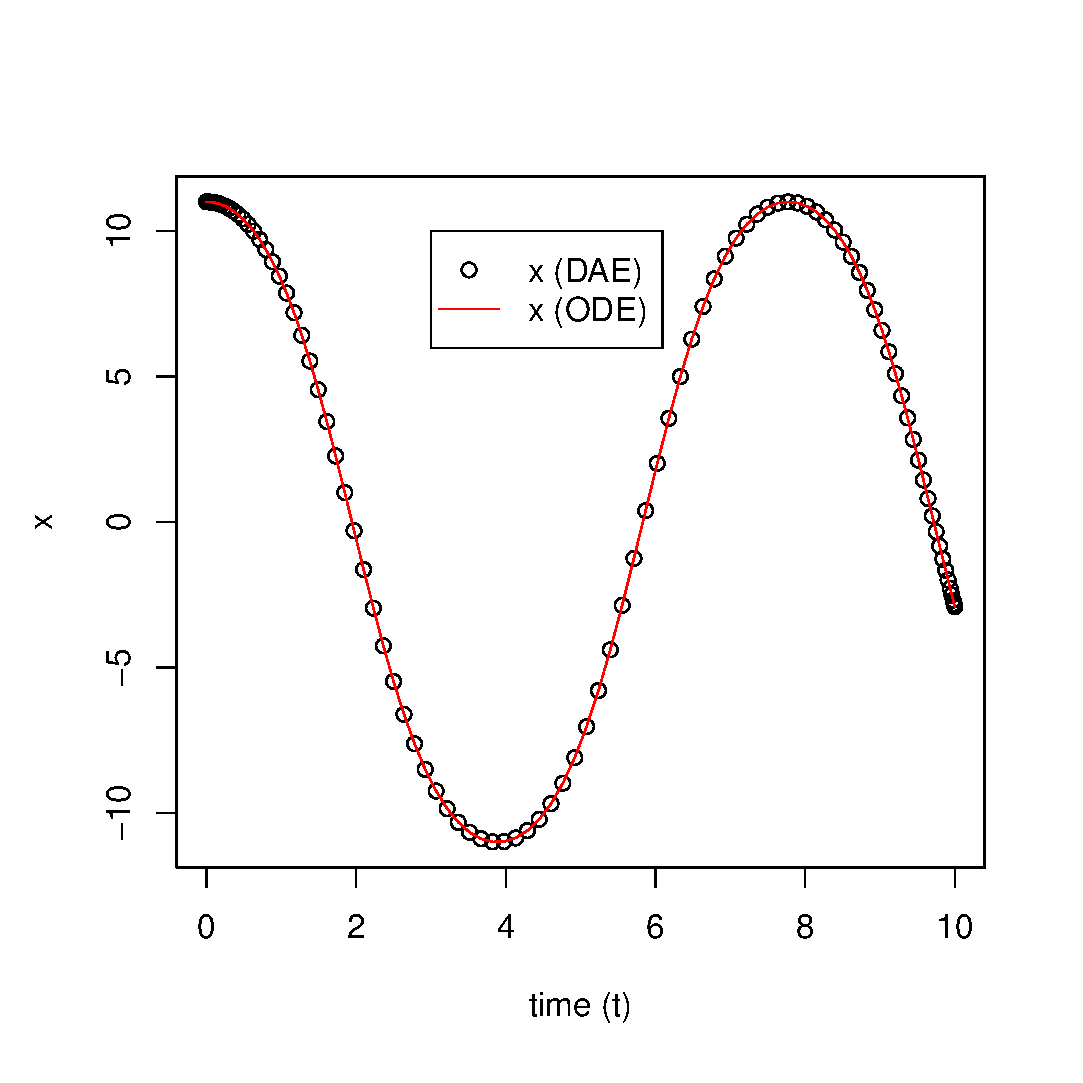
\includegraphics[width = 0.6\textwidth]{x.eps}
%	\end{center}
%\end{figure}
%\begin{figure}
%	\begin{center}
%		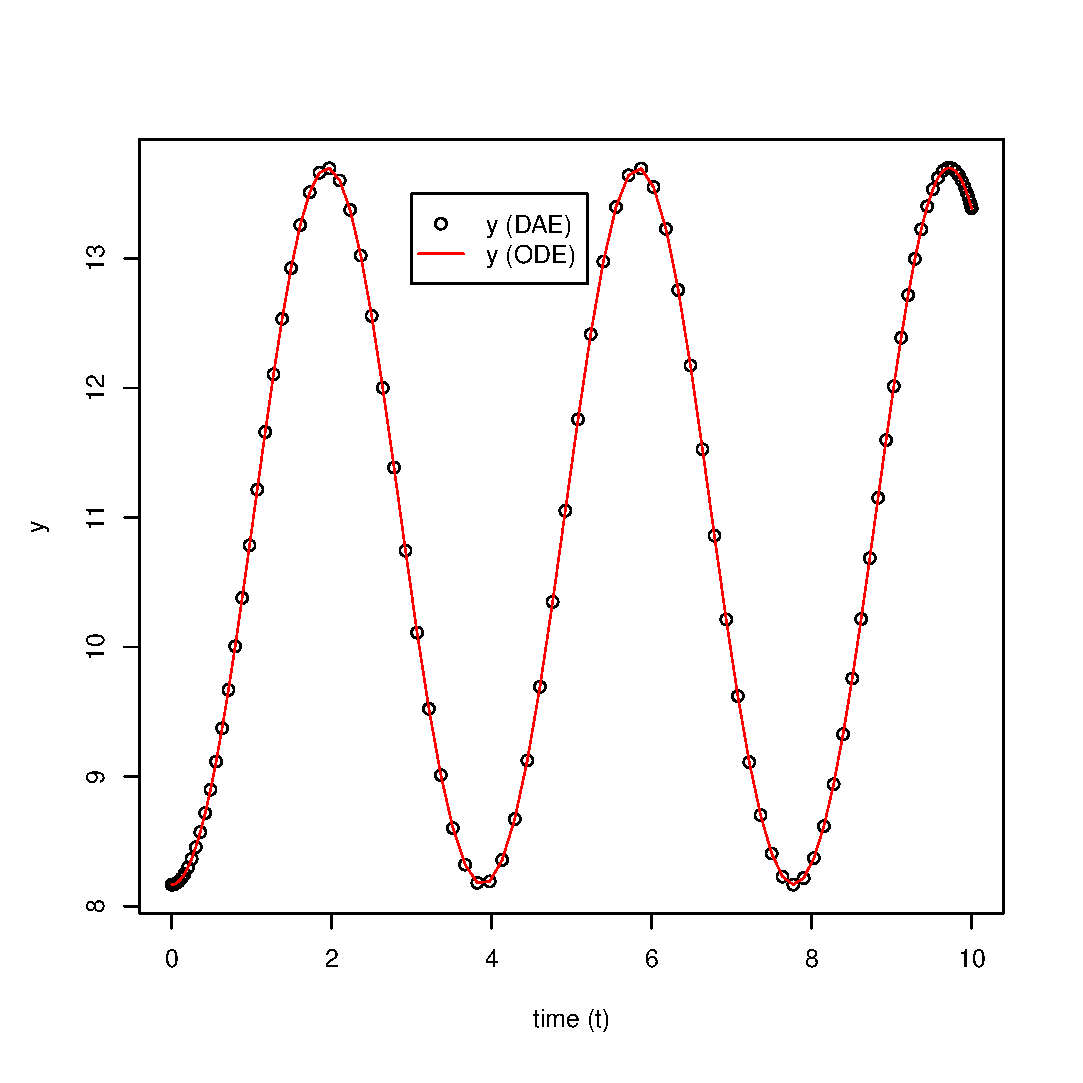
\includegraphics[width = 0.6\textwidth]{y.eps}
%	\end{center}
%\end{figure}
%%\begin{figure}
%	\begin{center}
%		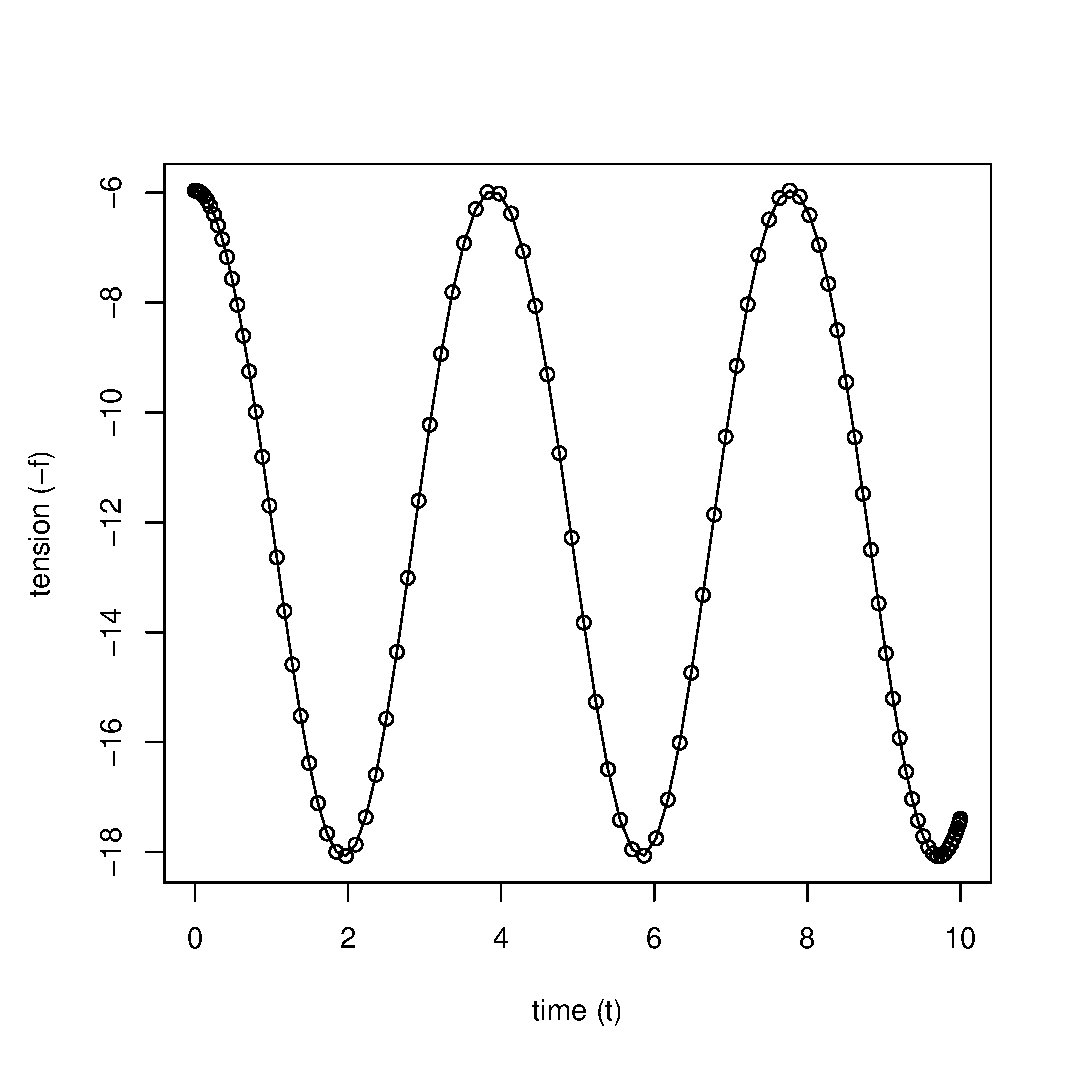
\includegraphics[width = 0.5\textwidth]{f.eps}
%	\end{center}
%\end{figure}

\end{document}